\documentclass[tikz,border=12pt]{standalone}
% Match the sans-serif font stack used by the Minimal Mistakes site theme.
% TeX Gyre Heros is the TeX-compatible Helvetica implementation.
\usepackage[T1]{fontenc}
\usepackage{tgheros}
\renewcommand{\familydefault}{\sfdefault}

\usetikzlibrary{arrows.meta,positioning}
\definecolor{pink}{HTML}{F72585}\definecolor{blue}{HTML}{4DABF7}\definecolor{green}{HTML}{51CF66}
\definecolor{red}{HTML}{FF6B6B}\definecolor{ink}{HTML}{E9ECEF}\definecolor{panel}{HTML}{211C1D}
\begin{document}
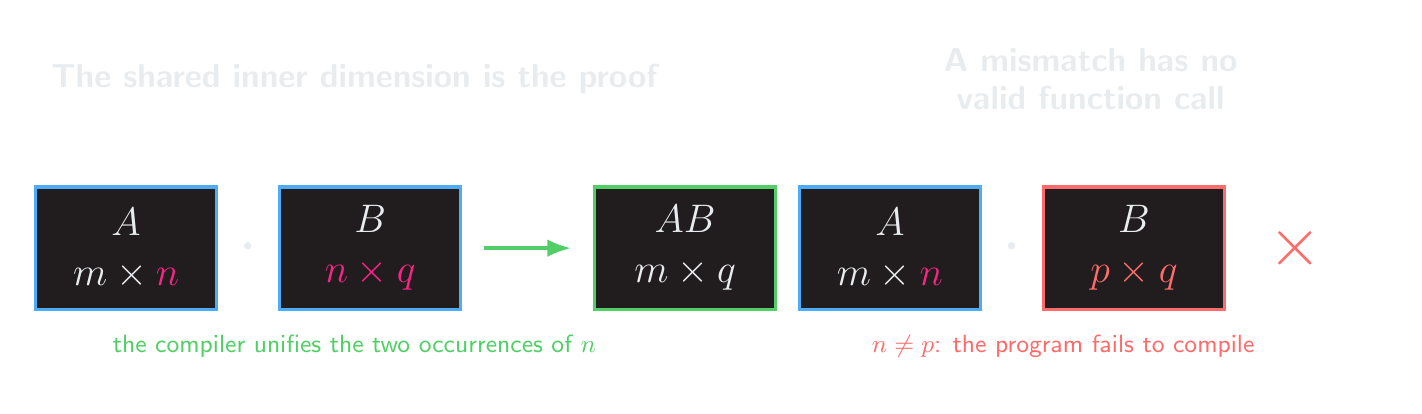
\begin{tikzpicture}[text=ink,matrix/.style={draw=blue,fill=panel,very thick,minimum width=2.3cm,minimum height=1.55cm,align=center,font=\Large},arrow/.style={-{Latex[length=3mm]},very thick}]
 \path[use as bounding box] (-1.25,-1.75) rectangle (16.1,2.8);
 \node[font=\bfseries\large,text=ink] at (2.9,2.15) {The shared inner dimension is the proof};
 \node[matrix] (a) at (0,0) {$A$\\$m\times\color{pink}{n}$};
 \node[font=\Huge] at (1.55,0) {$\cdot$};
 \node[matrix] (b) at (3.1,0) {$B$\\$\color{pink}{n}\times q$};
 \draw[arrow,green] (4.55,0)--(5.65,0);
 \node[matrix,draw=green] at (7.1,0) {$AB$\\$m\times q$};
 \node[font=\small,text=green] at (2.9,-1.25) {the compiler unifies the two occurrences of $n$};
 \begin{scope}[xshift=9.7cm]
  \node[font=\bfseries\large,text=ink,align=center,text width=6cm] at (2.55,2.15) {A mismatch has no valid function call};
  \node[matrix] at (0,0) {$A$\\$m\times\color{pink}{n}$};
  \node[font=\Huge] at (1.55,0) {$\cdot$};
  \node[matrix,draw=red] at (3.1,0) {$B$\\$\color{red}{p}\times q$};
  \node[font=\Huge,text=red] at (5.15,0) {$\times$};
  \node[font=\small,text=red] at (2.2,-1.25) {$n\neq p$: the program fails to compile};
 \end{scope}
\end{tikzpicture}
\end{document}
